\section{Ziel}
\label{sec:Ziel}
Ziel des Versuchs ist die Vermessung und anschließende Analyse der Magnetfelder verschiedener Spulen. Betrachet werden eine "lange" \: Spule, ein Helmholtzspulenpaar und eine 
Toroidspule. Eine Spule wird als lange Spule bezeichnet, wenn die Länge im Vergleich zum Spulen Durchmesser groß ist.
Es sollen der Verlauf der Magnetfeldstärke der ersten beiden Spulen und die Hysteresekurve des Kernmaterials der Toroidspule untersucht werden.

\section{Theorie}
\label{sec:Theorie}
Bewegen sich Ladungen im Raum, verursachen diese Magnetfelder. So ensteht um einen stromdurchflossenen Leiter ein stationäres Magnetfeld, welches proportional zum Strom 
$I$ des Leiters ist. Die Stärke dieses Magnetfeldes wird mit $\vec{H}$ bezeichnet. Mit der Magnetfeldstärke lässt sich wiederum die magnetische Flussdichte $\vec{B}$ als 
\begin{equation*}
    \vec{B} = \mu_0 \mu_r \vec{H}
\end{equation*} 
berechnen. Die Konstante $\mu_0$ wird als \textit{magnetische Feldkonstante} bzw. \textit{Vakuum-Permabilität} bezeichnet. Der zweite Faktor $\mu_r$ ist die relative Permabilität,
welche von dem Material abhängt, in dem sich das Magnetfeld befindet. 

\subsection{Magnetfelder von Spulen}
\label{subsec:Spulen}
Die Flussdichte $\vec{B}$ lässt sich dann im Vakuum mit dem \textit{Biot-Savartschen Gesetz}
\begin{equation}
    \label{eqn:BiotSavart}
    \symup{d} \vec{B} = \frac{\mu_0 I}{4 \pi}\frac{\symup{d}\vec{s} \times \vec{r}}{r^3}
\end{equation}
durch Integration über die Leiterschleife berechnen, wobei $r$ den Abstand vom Leiter beschreibt. Für eine runde, geschlossene Leiterschleife ergibt sich so für das Magnetfeld
entlang der Symmetrieachse $X$
\begin{equation*}
    \vec{B}(x) = \frac{\mu_0 I}{2} \frac{R^2}{(R^2+x^2)^{3/2}} \cdot {\vec{e}_x}.
\end{equation*}
mit dem Radius $R$ der Leiterschleife.
Bei einer langgestreckten stromdurchflossenen Spule der Länge $l$ ergibt sich durch Überlagerung der Flussdichte von $N$ Leiterschleifen (Windungen) ein homogenes Magnetfeld mit 
Betrag
\begin{equation}
    \label{eqn:LangeSpule}
    B = \mu_r \mu_0 \frac{N I}{l}
\end{equation}
im Inneren der Spule. An den Rändern der Spule gilt dies nicht mehr. 
Um die Randeffekte zu elimiieren, kann die Spule zu einem Ring gebogen werden. Das Magnetfeld des so entstandenen Torus verhält sich im Inneren wie jenes einer langen Spule mit
Länge $l = 2\pi R$. Außerhalb des Torus ist das Magnetfeld konstant 0. 

Eine weitere Aufbau, mit dem ein homogenes Magnetfeld erzeugt werden kann, ist der des Helmholtzspulenpaares in \autoref{fig:HelmholtzSkizze}.
\begin{figure}{h}{3.5cm}
    \centering
    \caption{Geometrie eines Helmholtzspulenpaares. \cite{v308}}
    \label{fig:HelmholtzSkizze}
    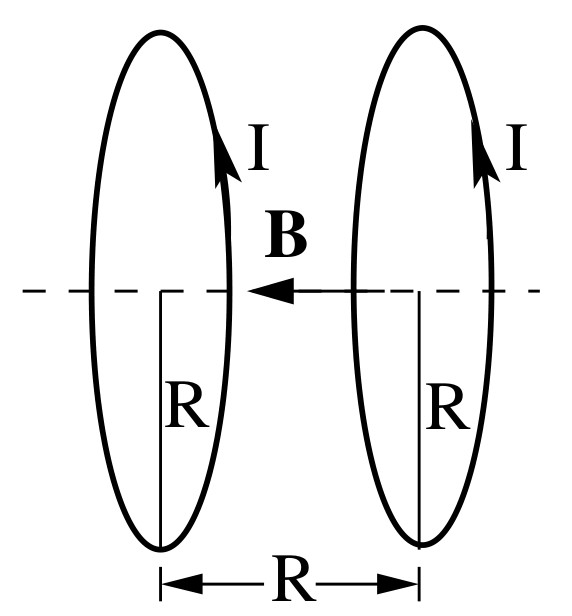
\includegraphics[width=3.5cm]{content/HelmholtzSkizze.jpg}
\end{figure}
Die Spulen sind parallel angeordnet und werden gleichsinnig vom Strom druchflossen. Der Abstand der Spulen sollte dem Spulenradius $R$ entsprechen. Bei einer solchen Anordnung 
ist das Magnetfeld entlang der Symmetrieachse homogen. Falls sich der Abstand $d = 2x$ vom Spulenradius unterscheidet, gilt diese Homogenität nicht mehr. Das Magnetfeld im 
Zentrum eines Spulenpaars mit je einer Windung kann in diesem Fall durch Überlagerung der Felder $B_1$ der einzelnen Spulen als
\begin{equation}
    \label{eqn:Helmholtz}
    B(0) = B_1(x) + B_1(-x) = \frac{\mu_0 I R^2}{(R^2 + x^2)^{3/2}}
\end{equation}
bestimmt werden. Um die Flussdichte für $N$ Windungen pro Spule zu erhalten, kann \autoref{eqn:Helmholtz} mit $N$ multipliziert werden. Es sei gesagt, dass so die Ausdehnung
der Spulen nicht berücksichtigt wird, was jedoch in der Praxis ohnehin vernachlässigt werden kann. % Lässt sich drüber streiten ob das n bissl shady ist 
Auch der Feldgradient $\frac{\symup{d}B}{\symup{d}x}$ ist im Idealfall in einem relativ großen Bereich vernachlässigbar gering.

\subsection{Magnetisierung ferromagnetischer Stoffe}
\label{subsec:Hysterese}
